\documentclass[review]{elsarticle}

\usepackage{lineno,hyperref}
\modulolinenumbers[5]

\graphicspath{ {./figures/} }

\journal{IB200}

%%%%%%%%%%%%%%%%%%%%%%%
%% Elsevier bibliography styles
%%%%%%%%%%%%%%%%%%%%%%%

%% Harvard
\bibliographystyle{model2-names}\biboptions{authoryear}

%% `Elsevier LaTeX' style
%\bibliographystyle{elsarticle-num}

%%%%%%%%%%%%%%%%%%%%%%%

\begin{document}

\begin{frontmatter}

\title{Fossil-calibrated phylogeny and chromosome evolution of Onagraceae}

\author[berk]{William A. Freyman\corref{cor1}}
\ead{freyman@berkeley.edu}
\cortext[cor1]{Corresponding author}

\address[berk]{Jepson Herbarium and Department of Integrative Biology, University of California, Berkeley}

\begin{abstract}
This template helps you to create a properly formatted \LaTeX\ manuscript.
\end{abstract}

%\begin{keyword}
%\texttt{elsarticle.cls}\sep \LaTeX\sep Elsevier \sep template
%\MSC[2010] 00-01\sep  99-00
%\end{keyword}

\end{frontmatter}

\linenumbers

\section{Introduction}

blah blah

\section{Methods}

\paragraph{Supermatrix} 

1: Downloads GenBank database of the specified GB division (PLN, MAM, etc)
2: Perform exhaustive all-by-all BLAST comparisons of each ingroup and outgroup sequence.
3: Alternatively (much faster) uses a FASTA file of guide sequences to define each cluster.
   Each ingroup/outgroup sequence is BLASTed against the guide sequences.
   4: Build clusters of sequences:
           - use single-linkage hierarchical clustering algorithm
	           - distance threshold default BLASTn e-value 1.0e-10
		           - uses sequence length percent similarity cutoff default 0.5
			           - discards clusters that are not phylogenetically informative (< 4 taxa)
				   5: Aligns each cluster of sequences using MUSCLE.
				   6: Concatenates the clusters creating a supermatrix.


\paragraph{Phylogenetic analysis} Once the package is properly installed, you can use the document class \emph{elsarticle} to create a manuscript. Please make sure that your manuscript follows the guidelines in the Guide for Authors of the relevant journal. It is not necessary to typeset your manuscript in exactly the same way as an article, unless you are submitting to a camera-ready copy (CRC) journal.

\paragraph{Chromosome evolution} The Elsevier article class is based on the standard article class and supports almost all of the functionality of that class. In addition, it features commands and options to format the
\begin{itemize}
\item document style
\item baselineskip
\item front matter
\item keywords and MSC codes
\item theorems, definitions and proofs
\item lables of enumerations
\item citation style and labeling.
\end{itemize}

\section{Results}

The author names and affiliations could be formatted in two ways:
\begin{enumerate}[(1)]
\item Group the authors per affiliation.
\item Use footnotes to indicate the affiliations.
\end{enumerate}
See the front matter of this document for examples. You are recommended to conform your choice to the journal you are submitting to.

\begin{figure*}[t]
    \centering
    % have to trim bottom off image
    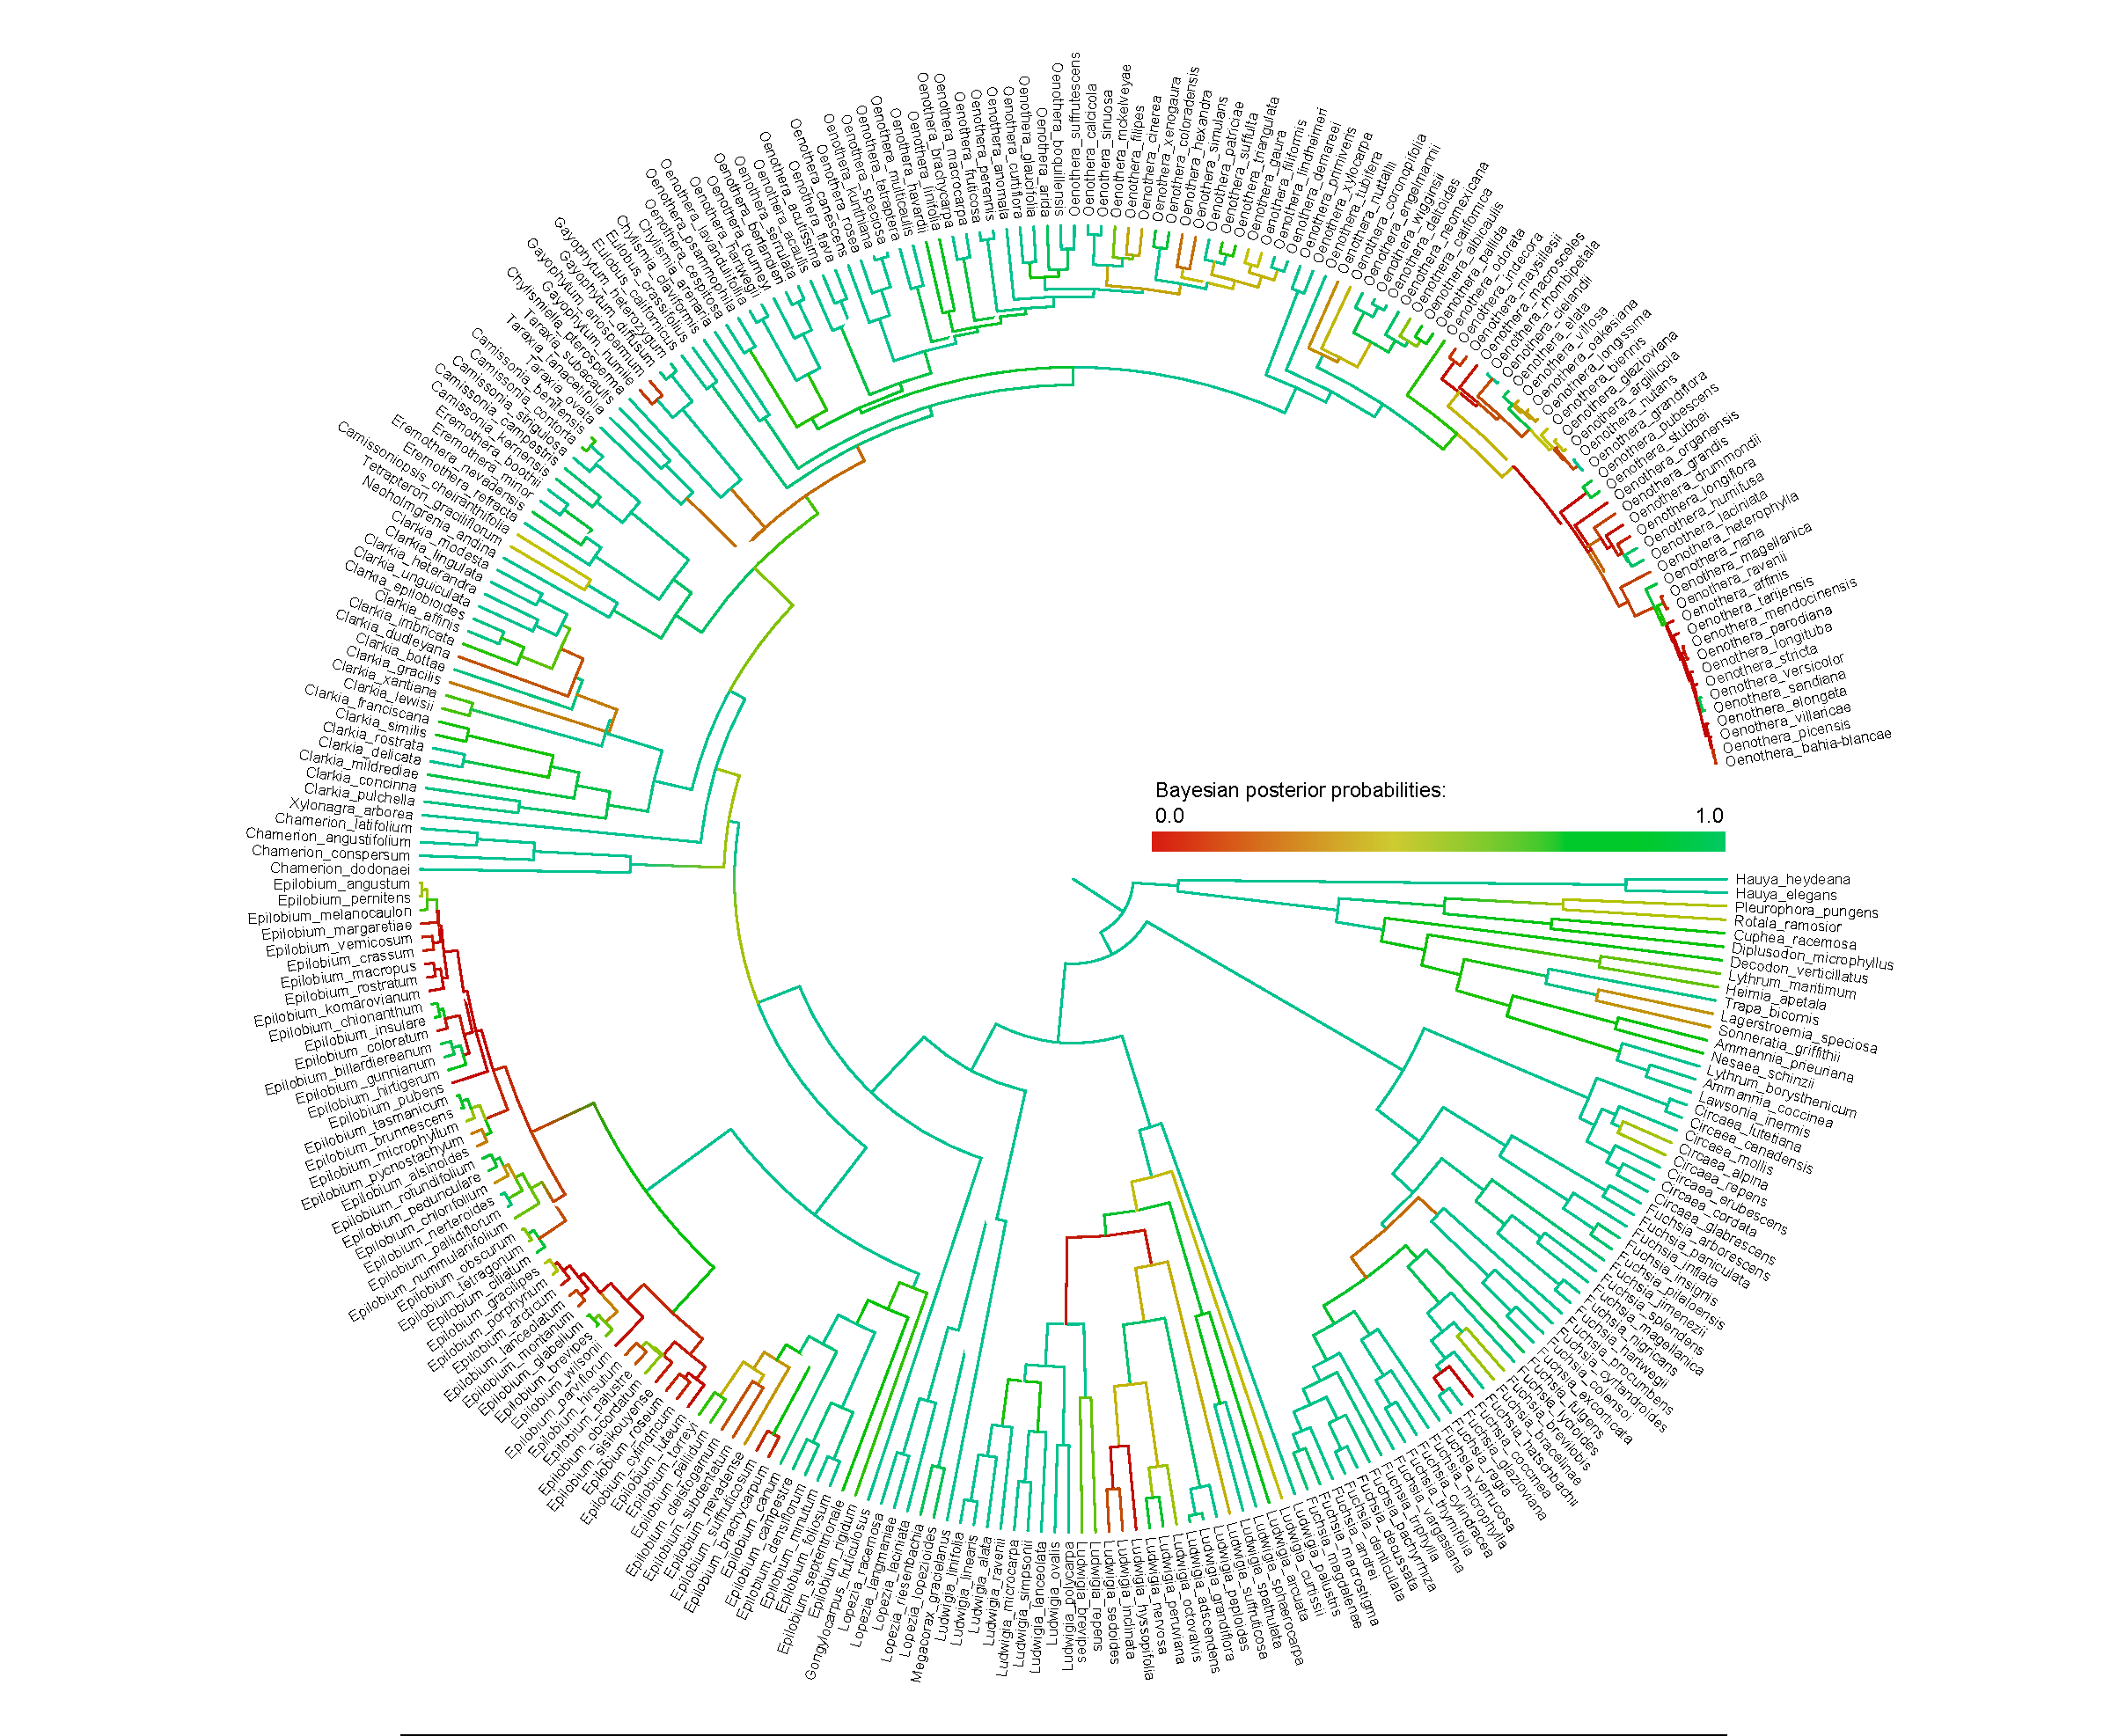
\includegraphics[width=1.0\textwidth, trim=0 10 0 0, clip=true]{colored_posterior}
    \caption{Phylogeny blah blah blah}
    \label{posteriors}
\end{figure*}

\begin{figure*}[t]
    \centering
    % have to trim bottom off image
    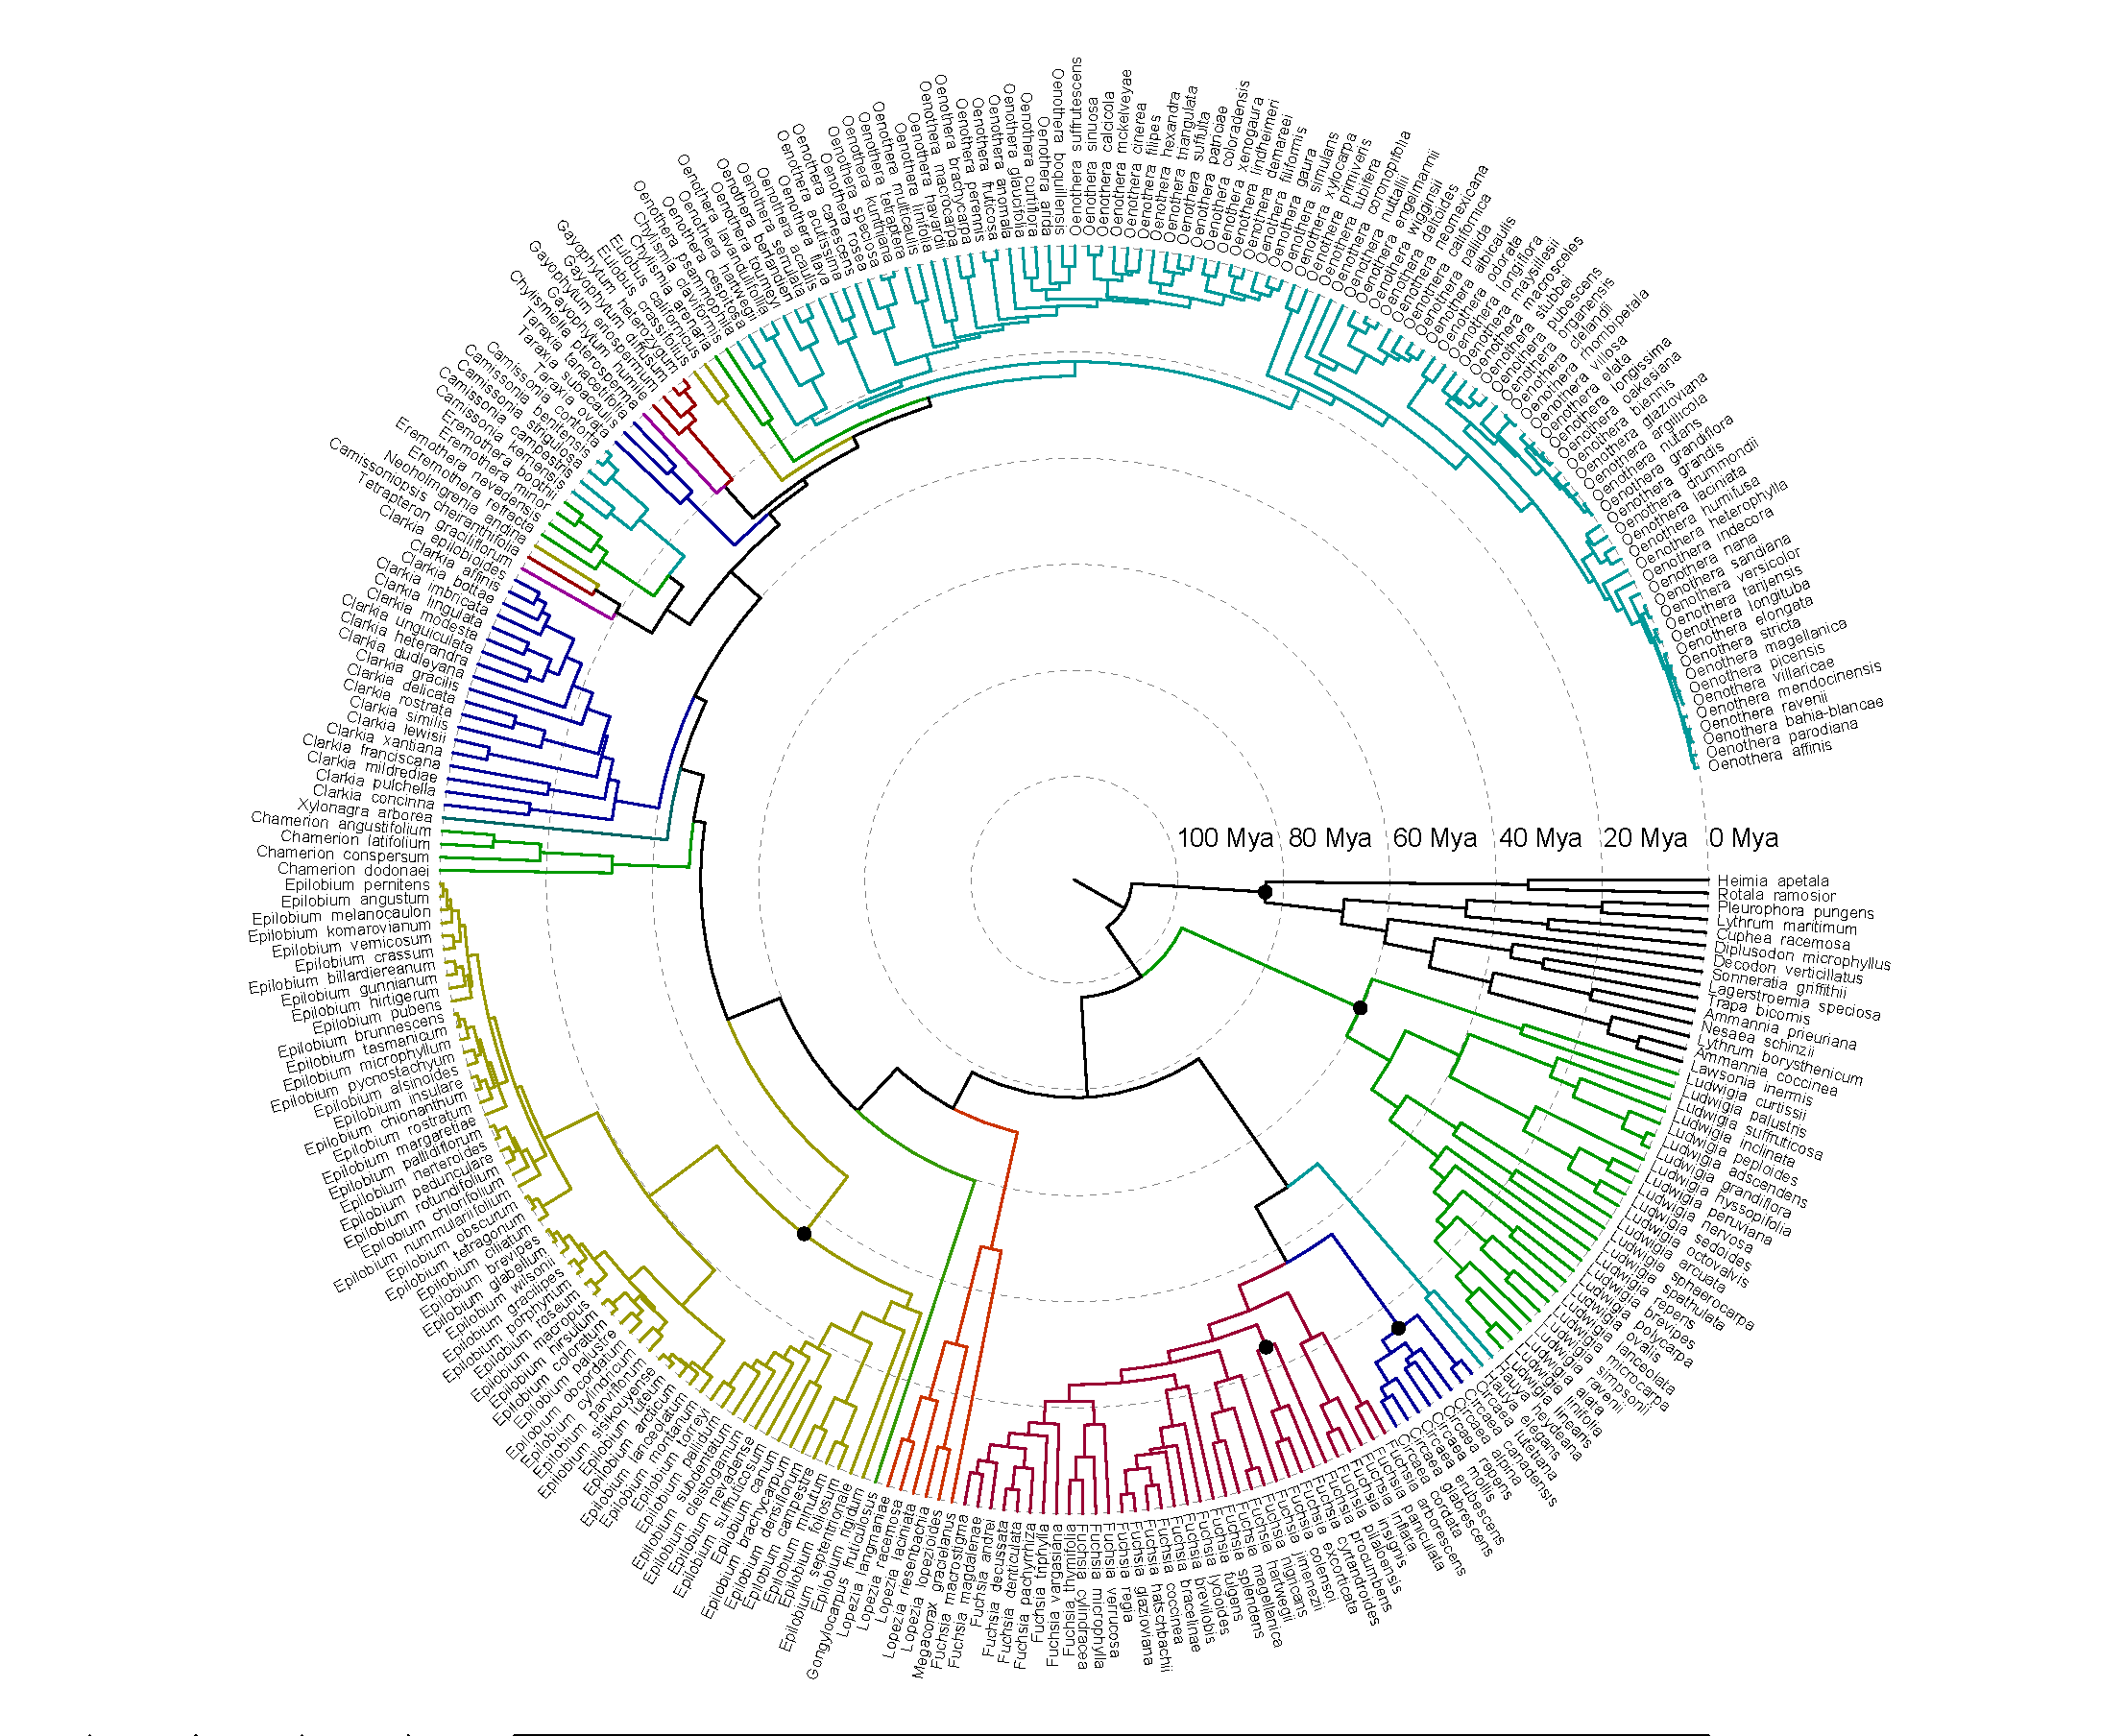
\includegraphics[width=1.0\textwidth, trim=0 10 0 0, clip=true]{time_colored_genera}
    \caption{Phylogeny blah blah blah}
    \label{genera}
\end{figure*}


\section{Conclusion}

There are various bibliography styles availablei, please see Figure \ref{genera}. You can select the style of your choice in the preamble of this document. These styles are Elsevier styles based on standard styles like Harvard and Vancouver. Please use Bib\TeX\ to generate your bibliography and include DOIs whenever available.

Here are two sample references: \citep{Feynman1963118,Dirac1953888}.

\section*{References}

\bibliography{manuscriptbib}

\end{document}
